\chapter{Design of Distributed Vision-based Control}


\section{Design approach}

The basic “system” is comprised of the QBot2 Mobile Robot and QUARK Control Software on a host computer.  The full “system” is comprised of multiple QBot2s collaboratively tracking a single target with the Quark Control Software Computer.  Note: An assumption is that the Quark Control Software on the host computer could be ported entirely to the robots, given sufficient processing and communications, to attain higher autonomy and actual decentralization of the system.  The target in the experiment is a round ball that is detected, located, and tracked by the multiple QBot2s.    
Subsystems for the basic system, a single QBot2, include: the Qbot2 mechanical/motors/control subsystem, the sensing/image processing subsystem, and the communications/processing subsystems (on the Qbot2 and the Host computer). 

\section{QBot2 Mobile Robot and QUARC Platform}

The QBot2 utilizes QUARC’s HIL software suite to allow users to design their program using Matlab and Simulink.  The Simulink model and Matlab code are translated to C++ code by the QUARC software and compiled automatically on the Qbot2’s computer.

\subsection{Hardware}

The QBot2 comes equipped with a differential drive robot base which has a maximum speed of 0.7m/s. A v1 Kinect-for-Xbox mounted on the robot base provides both color and distance vision information.  The RGB image that has a default resolution of 640 × 480 pixels and a 57° × 43° field of view.  The depth image has a resolution of 640 × 480 pixels, approximately 52.5° × 41° field of view, and measures distances from 0.5m to 6.0m. It is worth noting that the accuracy of the depth map depends on the detail of the grid projected by the IR emitter, the actual accuracy of the depth image is significantly lower than a resolution of 640x480 implies.   QBots use IEEE 802.11 b/g/n protocol for communication between the computer and QBot2. TCP/IP protocol is utilized, with each QBot2 using a statically assigned IP address. More information on sensors can be found in the appendix.

\begin{figure}[htbp] %  figure placement: here, top, bottom, or page
     \centering
     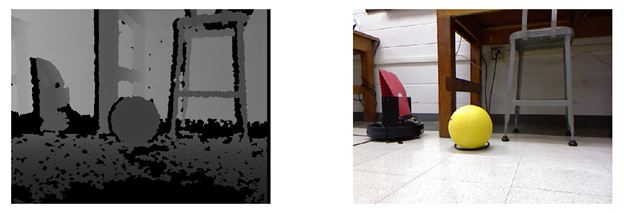
\includegraphics[width=5in]{1.png} 
     \caption{Side-By-Side of Color and Depth Images}
     \label{fig:1}
  \end{figure}     


\begin{figure}[htbp] %  figure placement: here, top, bottom, or page
     \centering
     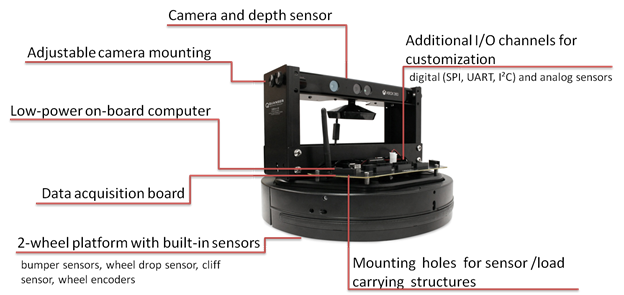
\includegraphics[width=4in]{2.png} 
     \caption{QBot2 Mobile Robot}
     \label{fig:2}
  \end{figure}     


\subsection{Software}
To connect to the QBOT2 A host-target real-time control system [2] is utilized.   As shown in Figure 3-2, the target QBOT2 computer is connected wirelessly with the host computer on which the SIMULINK model is running. The control algorithms are developed in MATLAB/SIMULINK with QUARC on the host computer. The control models are cross-compiled and downloaded to the target computer in real time. 


\begin{figure}[htbp]
\begin{center}
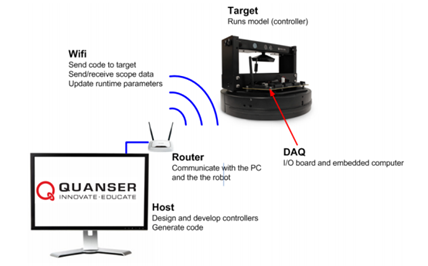
\includegraphics[width=5in]{3}
\caption{Host Computer / Wi-Fi Router to Qbot Communications Connectivity} \label{fig:3}
\end{center}
\end{figure}

\section{Target Identification}
\subsection{Interface and inputs to Target Control}
The result of the vision control system is a target location given in 2D Cartesian coordinates. The origin of this coordinate plane is at the Qbot2’s camera position, the positive X axis extends in same the direction the Kinect is facing and the positive Y axis extends to the left (or “port” side) of the Kinect.  The motion control module will then transform this point according to its current kinematic state.   This is target point is the basic interface between the target identification module and the motion control.

Based on the 2016 Senior Project, and research of alternatives, we chose to use the color image for object/target recognition and the depth image for determining distance to the target. Our choice was driven primarily by practical QBot2 processing limitations and timing restrictions prohibiting potentially more robust methods of object detection (see Appendix).

\subsection{Acquire Y Component of Target Location from Color Imagel}
We perform all object recognition on the color image.  Consequently, color image processing is the primary bottleneck in system performance.  We initially selected color thresholding with blob detection because it is the easiest image processing method to implement.  Although we did pursue alternative methods of image processing, these implementations were unable to meet our performance requirements due to limitations of the Qbot2 hardware.  Therefore, color thresholding with blob detection was selected because it had a significantly lower performance requirement while also producing adequate results. 

The first stage of image processing, color thresholding, highlights all elements of the image that correspond to our target’s color.  During this stage, pixels with RGB values that fall within a pre-determined range are replaced by ‘1’ in the binary output image, while all other values are replaced by ‘0’.  

Blob detection is applied to the binary output image from color thresholding.  The goal is to identify the largest grouping of neighboring, non-zero values.  Then, for each group (or “blob”) of neighboring pixels, we calculate its centroid by finding the mean index of all pixels contained in that blob.  This means that the accuracy of the blob corresponding to our target object is unaffected by “noise” from similar colors appearing elsewhere in the image.  It should be noted that the accuracy of this method is therefore entirely dependent on the color thresholding result.  

\begin{figure}[htbp]
\begin{center}
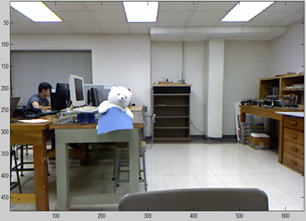
\includegraphics[width=5in]{4}
\caption{Before Processing - Color Thresholding and Blob Detection} \label{fig:4}
\end{center}
\end{figure}

\begin{figure}[htbp]
\begin{center}
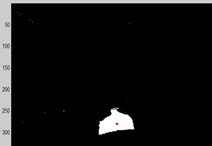
\includegraphics[width=5in]{5}
\caption{After Processing - Color Thresholding and Blob Detection} \label{fig:5}
\end{center}
\end{figure}
The blob detection outputs a list of centroids and corresponding blob sizes.  If the blob size of the largest blob is greater than some pre-determined threshold value, our system will use that centroid for the target’s coordinates on the RGB image plane. 


\subsection{Acquire X Component of Target Location from Depth Image}
The target’s location on the depth map can be estimated by translating points from the color image plane to the depth image plane.  We calculated this using the ratio between the two images’ field-of-view and the estimated angle from the RGB image.

\begin{figure}[htbp]
\begin{center}
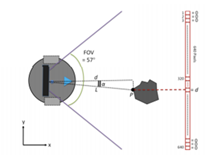
\includegraphics[width=5in]{6}
\caption{Target Localization} \label{fig:6}
\end{center}
\end{figure}

\begin{equation}
∝_T=(L_{color}/2-X_{color} )(¬(FOV_{color}-x)/L_{color} )
\end{equation}

\begin{figure}[htbp]
\begin{center}
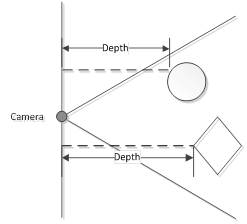
\includegraphics[width=5in]{7}
\caption{Host Computer / Wi-Fi Router to Qbot Communications Connectivity} \label{fig:7}
\end{center}
\end{figure}

\begin{equation}
〖XY〗_{depth}=(〖FOV〗_{color}/L_{color} )(L_{depth}/〖FOV〗_{depth} ) 〖∙XY〗_{color}+offset
\end{equation}
\begin{equation}
X_T=〖Image〗_{depth} (X_{depth},Y_{depth})
\end{equation}
\begin{equation}
Y_T=X_T∙tan⁡(∝_T)
\end{equation}
\section{Motion Control}
\subsection{Encirclement}
The target control module relies on received target coordinates from the image processing module and the robot’s  x,y, and theta. These are inputs which allow for formulation of encirclement.  From the robot’s x,y, and theta values, we transform these values to the appropriate kinematic model for the QBot2. From this kinematic model, we transform the cartesian local coordinate system to a cylindrical coordinate system. The length between the two wheels of the QBot is 0.0235 meters. To find the forward point location of the robot, we use,
\begin{equation}
	P_x=x+0.0235*cos⁡(θ)
\end{equation}
\begin{equation}
	P_y=y+0.0235*sin⁡(θ)
\end{equation}

Following, we want to define qi,
\begin{equation}
	q_i=〖(ρ〗_i  ϕ_i)
\end{equation}
	
and convert these values by,
\begin{equation}
	ρ(p)=√((p_x^2+p_y^2 ) )
\end{equation}
	
\begin{equation}
	ϕ(p)=〖atan〗^2⁡〖〖(P〗_y,Px) 〗
\end{equation}
	

where p is the pose of the model.

ρ ̇ and ϕ ̇ are the forward velocity and angular velocity computed by:
----
\begin{equation}
	ρ ̇=k_r*(ρ_s- ρ_d)	(6)
\end{equation}
		
\begin{equation}
	ϕ ̇=ω_d
\end{equation}
	

where $k_r$  is the porportional gain and $ρ_s$ is the size of the encirclement radius. $ρ_d$ is the approximate distance from the robot to the target given from the inverse kinematics and image processing modules.

We then use the Jacobian matrix of the difference between the target and robot where Px and Py is the X and Y coordinates of the robot and Pxt and Pyt is the X and Y coordinates of the target in relation to the robot’s coordinate frame. The difference of the robots X and Y locations can be reduced to Pxd and Pyd. and the following Jacobian  matrix can be computed
\begin{equation}
		J_i=((P_xd/√(P_xd^2+P_yd^2 )  P_yd/√(P_xd^2+P_yd^2 )  〖-P〗_yd/(P_xd^2+P_yd^2 )P_xd/(P_xd^2+P_yd^2 )))   
\end{equation}


	


From the Jacobian, the following input velocities Ux and Uy can be computed
\begin{equation}
		[U_x,U_y ]=J_i^(-1)*[ρ ̇,ϕ ̇]
\end{equation}
	
For the velocity inputs, $U_x$ and $U_y$ , they are transformed using the inverse kinematic equations
\begin{equation}
			p^(-1)=((cos⁡(θ)-0.0235*sin⁡(θ)@sin⁡(θ)0.0235*cos⁡(θ) ))^(-1)
\end{equation}
	

to find $V_c$ and $ω_c$,
\begin{equation}
[V_c,ω_c ]=p^(-1)*[U_x,U_y]
\end{equation}	

Once $V_c$ and $W_c$ are found, using
\begin{equation}
V_r=V_c+1/2* .0235*2*W_c
\end{equation}
\begin{equation}
	V_L=V_c-1/2* .0235*2*W_c
\end{equation}
	

	
we can find velocities of the right and left wheels, Vr and VL.

Right and left wheel velocities are then sent to the HIL Write block which sends data to the 2000 and 2001 ports of the QBot2 for the left and right wheels, respectively.
The QBot2 stores wheel encoder data to allow calculation of actual right and left wheel velocities. This data is taken from the HIL Read block. For each wheel encoder ticks, we can determine the velocity of each wheel. The robot’s x,y, and θ values are then updated and sent back into the control module using Vc and θ where,
\begin{equation}
V_c=0.5*(V_L+V_r)
\end{equation}
\begin{equation}
Θ=1/0.235*(V_r-V_L)
\end{equation}
	

	


From $V_c$ and $ω_c$, we can determine the robot’s X, Y, and θ values by calculating the integrals for
\begin{equation}
x ̇=cos⁡(θ)*V_c
\end{equation}
\begin{equation}
y ̇=sin⁡(θ)*V_c
\end{equation}
\begin{equation}
	θ̇=ω	
\end{equation}

	

		

\subsection{Encirclement}
Leader-follower control module is used for distributed multi-robot coordination. The leader-follower control module does not take into account inverse kinematics. And, the image processing is used to localize the leader robot coordinates ($𝑥_𝑟$  , $𝑦_𝑟$) in the vision sensor range. Given the radial distance of the target, $V_c$ and $ω_c$ are calculated. A follow distance of 0.5 meters and gains  Kw = 0.5 and Kv = 0.2 were defined as per limitations for the QBot.
To determine $V_c$ and $ω_c$,
\begin{equation}
	V_c=K_v*√(x_t^2+y_t^2 )-0.5	(15)
\end{equation}

\begin{equation}
	ω_c=-K_w*arctan⁡(x_t,y_t)
\end{equation}


where xt and yt are the positions of the target in relation to the robot’s local coordinate frame.
One should note the limits for angular and forward velocity are set to .2 m/s.



\section{Event-based System Control}
\subsection{Implementation}
The Simulink model is configured using the HIL block from the QUARC toolbox.  This enables users to more easily run their simulations in a virtual environment as well as on actual hardware.  The project must also be configured to communicate with a specific IP address, which can be done through the QUARC add-on options menu in Simulink.  It is also important to set the sample time configure the “Solver” pane of the Simulink model configuration.  It is important to select the “ode1” and “fixed-step” options.  Additionally, when performing operations on images or large arrays of data, it is recommended that users select a sample frequency no greater than 15Hz.  Our experiments used a 10Hz sample frequency.
\subsection{Tasks Coordination}
Our system would need to switch between two modes of operation depending on whether or not the target was in view.   Stateflow was used to control the varying states in our model. Models for both target encirclement and leader-follower used similar simulink and stateflow models with differences only in controls and how often a search was made. In both models, search mode is done by toggling between image processing and rotating. Once the desired accuracy is obtained from blob detection, the state switched to the control module.  The target encirclement model only searches for target every set time-interaction whereas leader-follower will search for a target every other time-step.

\begin{figure}[htbp]
\begin{center}
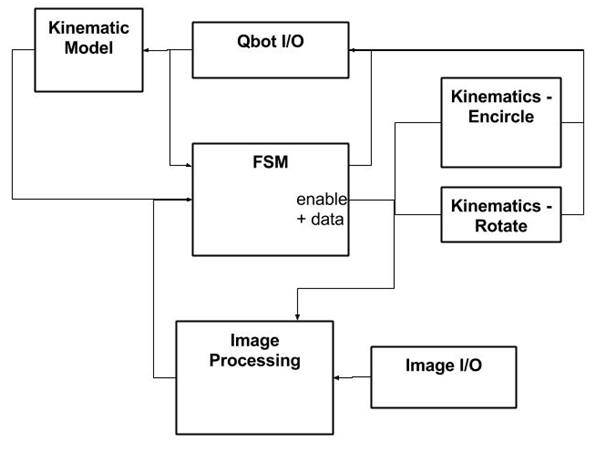
\includegraphics[width=5in]{8}
\caption{Abstracted View of Simulink Diagram} \label{fig:8}
\end{center}
\end{figure}

\subsection{Target Encirclement - Finite State Machine}
In the stateflow for target encirclement control, various enable switches allow triggering of different modules. The system starts off with all enable switches off. While entering target acquisition mode, image processing module is enabled and determines if an image centroid can be made. If no centroid is found, the QBot2 will rotate 15 degrees on its axis and wait for the cameras to update. If a centroid can be made, it checks whether the pixel size of the image is greater than a certain value. In our case, a yellow ball or box is used. If 30 pixels are connected, the robot will continue into the encirclement module. Data from the image processing, such as the robot’s x, y, and theta, is also sent to the encirclement module. From this module, the target location is stored and encirclement is based on this value. After 120 seconds, the encirclement ceases and target acquisition mode begins again

\begin{figure}[htbp]
\begin{center}
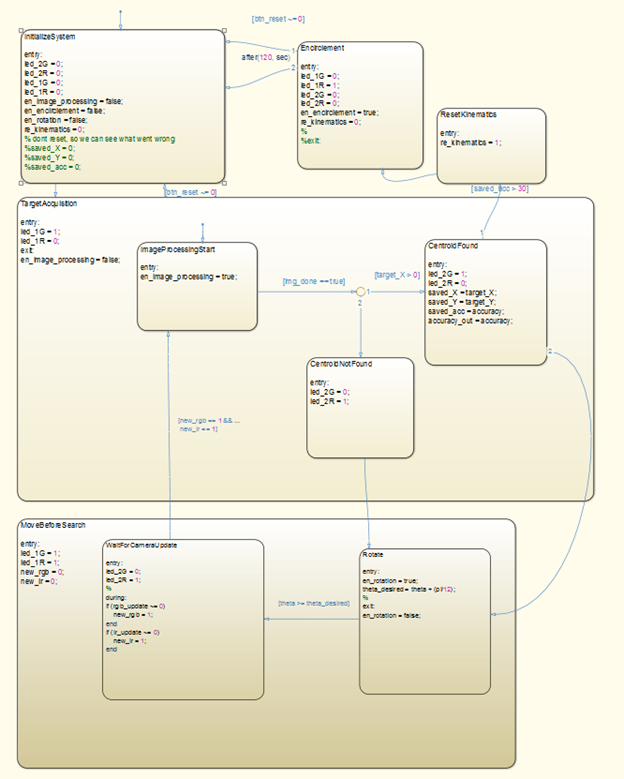
\includegraphics[width=5in]{9}
\caption{Event-based System Control: Encirclement Control} \label{fig:9}
\end{center}
\end{figure}

\subsection{Leader-Follower - Finite State Machine}

Leader-follower control is similar to target encirclement control. However, instead of returning to Target Acquisition mode, the target will continue to follow any centroid even if the pixel count is less than 30. The process is done by continually switching from image processing and the leader-follower control module. If no centroid is found, the target will return into Target Acquisition mode.


\begin{figure}[htbp] 
\begin{center}
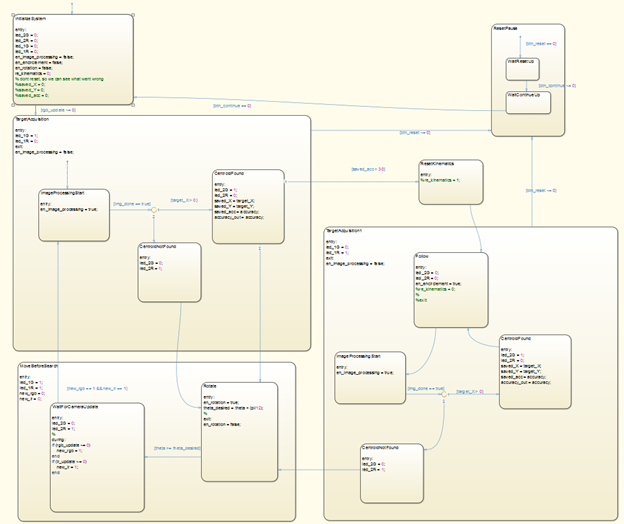
\includegraphics[width=5in]{10}
\caption{Event-based System Control:Ledaer-Follower Control} \label{fig:10}
\end{center}
\end{figure}


\section{Experiments}
A curriculum for the QBot was provided to allow interfacing and familiarity of the QBot2 and its software package, QUARC. The curriculum covers topics ranging from QBot communication, integration, kinematics and vision guided control. Advanced topics such as path planning, mapping, and localization are also covered. Each section provides an in-depth tutorial for the understanding of the QBot’s capabilities. Tutorials for blob detection, line-following, and kinematics were most referenced in our project.
Various simulations for the control module were implemented in Matlab and Simulink. These demonstrations assumed constant communication between robots. For encirclement control, single robot to a multiple robot models were simulated to show proof of concept. Refer to the appendix for more information.
From simulation, the first series of experiments were conducted. Using a predefined target point, encirclement of a single robot was tested. Our next iteration, using blob detection, allowed us to capture and encircle the target point. The next iteration consisted of determining which method of control was needed to allow coordination between robots. Stateflow was used to control different modules efficiently. Following, a leader-follower model was implemented for successive robots.

\section{Results}
Experimental results can be seen in figures below. Target encirclement was achieved by the target robot. Using the appropriate thresholds for the color yellow, the robot was able to identify the target.
\begin{figure}[htbp]
\begin{center}
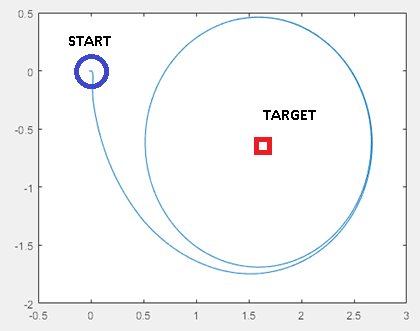
\includegraphics[width=5in]{11}
\caption{Phase Plot of Encirclement Robot} \label{fig:11}
\end{center}
\end{figure}

\begin{figure}[htbp]
\begin{center}
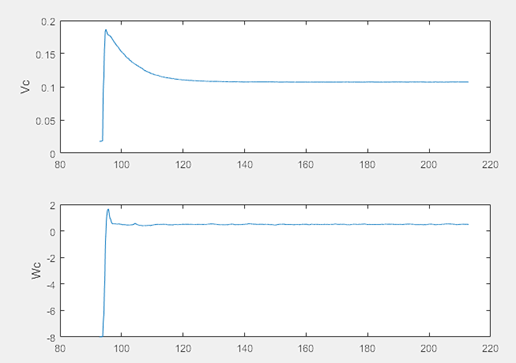
\includegraphics[width=5in]{12}
\caption{Forward and Angular Velocities of Encirclement Robot} \label{fig:12}
\end{center}
\end{figure}

\begin{figure}[htbp]
\begin{center}
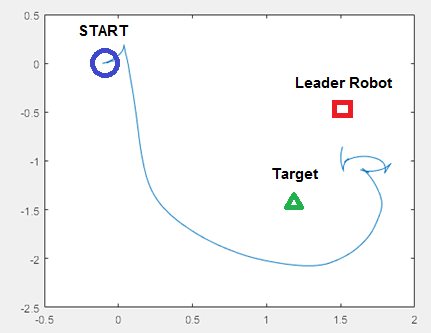
\includegraphics[width=5in]{13}
\caption{Phase Plot of Leader-Follower Robot} \label{fig:13}
\end{center}
\end{figure}

\begin{figure}[htbp]
\begin{center}
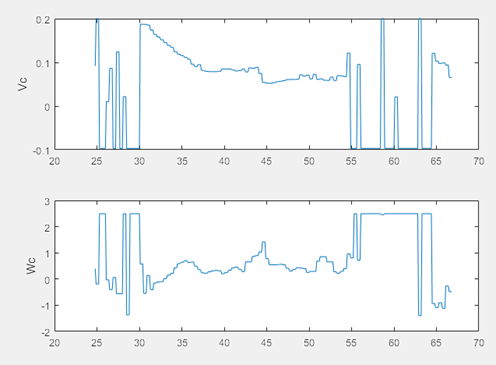
\includegraphics[width=5in]{14}
\caption{Forward and Angular Velocities of Leader-Follower Robot} \label{fig:14}
\end{center}
\end{figure}

Encirclement control can be seen in the following: https://www.youtube.com/watch?v=VHpTNNhiLG4
Leader-follower control can be seen in the following: https://www.youtube.com/watch?v=bO5DHXQCITw


